\documentclass[a4paper, twoside, 11pt]{article}
\usepackage[margin=1.5cm]{geometry}
\usepackage[]{xcolor}
\usepackage{cite}
\usepackage{graphicx}
\usepackage{listings}
\usepackage{float}
\usepackage{caption}
\usepackage{amsmath}

\usepackage{hyperref}

\hypersetup{
    colorlinks=true,
    linkcolor=blue,
    filecolor=magenta,      
    urlcolor=cyan,
}

\lstset{frame=tb,
  language=Java,
  aboveskip=3mm,
  belowskip=3mm,
  showstringspaces=false,
  columns=flexible,
  basicstyle={\small\ttfamily},
  numbers=none,
  numberstyle=\tiny\color{gray},
  keywordstyle=\color{blue},
  commentstyle=\color{dkgreen},
  stringstyle=\color{mauve},
  breaklines=true,
  breakatwhitespace=true,
  tabsize=3
}

\definecolor{dkgreen}{rgb}{0,0.6,0}
\definecolor{gray}{rgb}{0.5,0.5,0.5}
\definecolor{mauve}{rgb}{0.58,0,0.82}

% define the title
\author{L. ~Towell,\\ Student No: 201383538}

%defines the title
\title{Assignment 2\break Message Authentication \& Diffie-Hellman Key Exchange}

\begin{document}
	%generate the title
	\maketitle

\maketitle
\begin{center}
All programs and snippets are available in the below code repository. Please feel free to pull and execute the different applications.\\
Code repository: \href{https://github.com/luketowell/COMP522-Assignment2}{COMP522-Assignment 2}
\end{center}

\section{Comparison of Methods for Message Authentication}
\subsection{Hash-functions}
Hash functions are used in order to attempt to ensure to both the sender and the receiver that a message is authentic and has not been manipulated or interfered with in any way. Hash functions are typically used when a secret is not shared between the sender and the receiver. 
\\
The process of using a hash function is the following:\\
- An unencrypted message is sent from the sender to the receiver with a tag (hash) which has been generated by the sender.\\
- The receiver then receives the message and the tag and in order to establish if the message has been tampered with they generate their own hash using the plain text message from the sender.\\
- Once the receiver has generated their own hash they then compare the hash they generated to the hash they received as the tag. If the hash generated by the receiver doesn't match the tag hash then the message has been tampered with and the contents cant be trusted however if the hash and tag hash do match then the message hasnt been manipulated and can be trusted to be original.\\
\\
Hash functions are typically referred to as one way hashes. This is because it is easy to generate a hash using a message however it is very difficult to generate the message from the hash. The tag hash that is generated using a hash function algorithm e.g. the SHA1 typically produces a fixed length hash which is not dependent on the size of the message being sent.\\
\\
\textit{Appendix A} is an example of the SHA1 hash function which takes a string input and digests the input using the SHA1 algorithm to produce a byte array hash. See \textit{Figure 1} for the output of \textit{Appendix A.} 
\\
\begin{figure}[H]
	\centering
	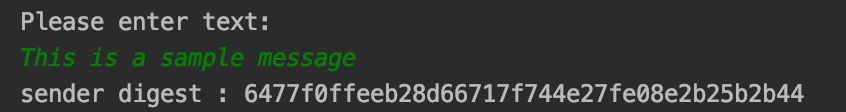
\includegraphics[scale=0.5]{Images/digestOutput.png}
  \caption{Output of non the hashing function}
\end{figure}
The advantage of hash functions are that they are very simple to compute and are an effective way of telling if a message is genuine or if it has been manipulated.\\
\\
The disadvantage of Hash functions are that since the message is unencrypted, the content of the message is not secure so anyone can read the original message and as long as they dont change the hash then the hash will still match the original message. The hash is also easy to replace so the message could be read and manipulated by an illicit party who could then generate a new hash tag and send the message on to the original recipient with a new content and a new hash which will match when they attempt to compare generated hashes. Hash functions however do not satisfy the weak and strong collision policys so it is possible you could generate a duplicate hash. Another issue with the SHA1 algorithm has been identified that it has a mathematical weakness which makes the outputs of the algorithm vulnerable to decryption.

\subsection{RSA + SHA1 method}
The methodology discussed in this section is the combination of the hashing mechanism SHA1 with the RSA algorithm which combines the hashing algorithm discussed previously in \textit{Section 1.1} and demonstrated in \textit{Appendix A} together with the use of public and private keys in order to create a more secure message sharing methodology. \\
\\
The combination of RSA and SHA1 hashing allows a sender (\textit{Appendix B}) to generate a hash using a hash algorithm e.g. SHA1 (\textit{Appendix A}). Then this hash tag is encrypted using a private key which has been generated as part of the key pair to produce a ciphertext.\\
\\
The ciphertext, plain text message and corresponding public key is sent to the verifier. (In the program provided in \textit{Appendix B \& Appendix C} the message has been abstracted into a Seperate object.)\\
\\
The verifier then uses the same hashing algorithm and the plain text message to generate their own hash. They also decrypt the ciphertext using the public key provided in the message. Once the verifier has their own hash and has the decrypted hash they can compare the values to see if they match. As in Hash functions if the hash tags do not match then the message is untrustworthy and needs to be discarded. \\
\\
An example of how a tampered with message can be detected can be created using \textit{Appendix B} and \textit{Appendix C}. In the experiment below I have generated a message containing the string "This is a sample message" which has then been encrypted and sent to the receiver class. However on the way to the varifier the message has been intercepted and the plain text has been changed to "This is not a sample message". As you can see from \textit{figure 3} below because the message has been changed the hash no longer matches and the message cannot be trusted. \textit{Figure 2} shows a successful message which has been received by the verifier without interference.

\begin{figure}[H]
	\centering
	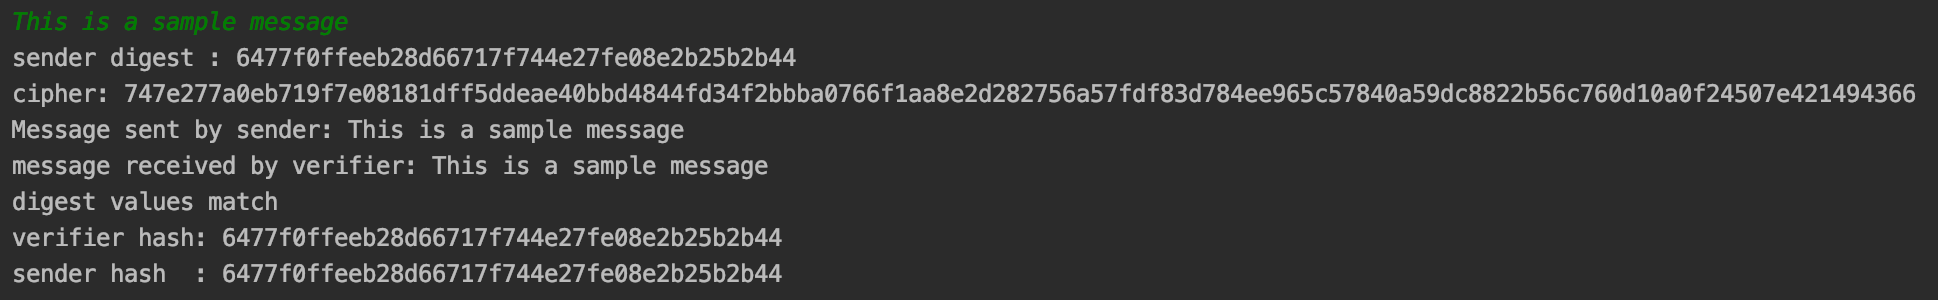
\includegraphics[scale=0.5]{Images/successMessage.png}
  \caption{Output of non intercepted message}
\end{figure}


\begin{figure}[H]
	\centering
	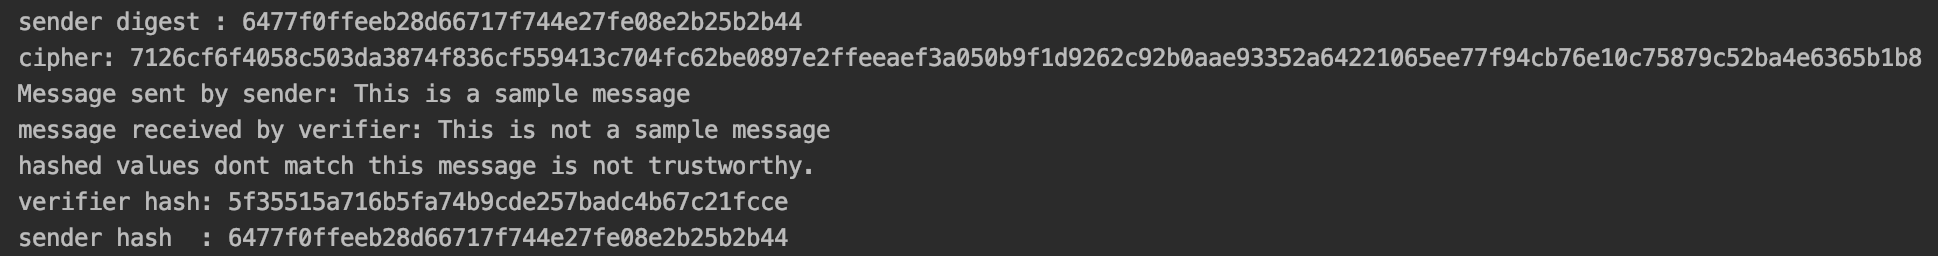
\includegraphics[scale=0.5]{Images/interceptedMessage.png}
  \caption{Output of intercepted message detection}
\end{figure}

\subsection{DSA (Digital Signature Algorithm) method}
The DSA methodology is Similar to the RSA + Hashing methodology however the DSA method does not encrypt the message hash like in the RSA methodology. The DSA method available in JPA performs the following steps:\\
 - Takes the original message from the sender, creates a hash and signs the message with a private key in order to create a signature that is unique to the message being sent.\\
- The message is then sent to the user which contains the original message, the signature hash that was generated by the sender and the public key of the sender.\\
- When the message is received by the verifier they are able to take the original message and generate a message hash.\\
- The received then takes their message hash and the senders public key and verifies that the public key being supplied is a match to the private key that was used to sign the content of the message.\\
- If the verify function of the DSA algorithm comes back as "True" then the message that has been received was the message that was sent and is genuine. If either the signature or the message has changed then the verify function will return false and the message can not be trusted as with all other message authentication methods already discussed. \\

The figures below show the results of experiments that have been ran on the DSA algorithm using the sender and verifier programs (\textit{Appendix D \& Appendix E}).\\
\\
\textit{Figure 4.} Shows that when the message is not intercepted and the original message and the signed hash are original then the DSA algorithm is able to run as expected and verify that the message has not been manipulated, meaning the message contents can be trusted.

\begin{figure}[H]
	\centering
	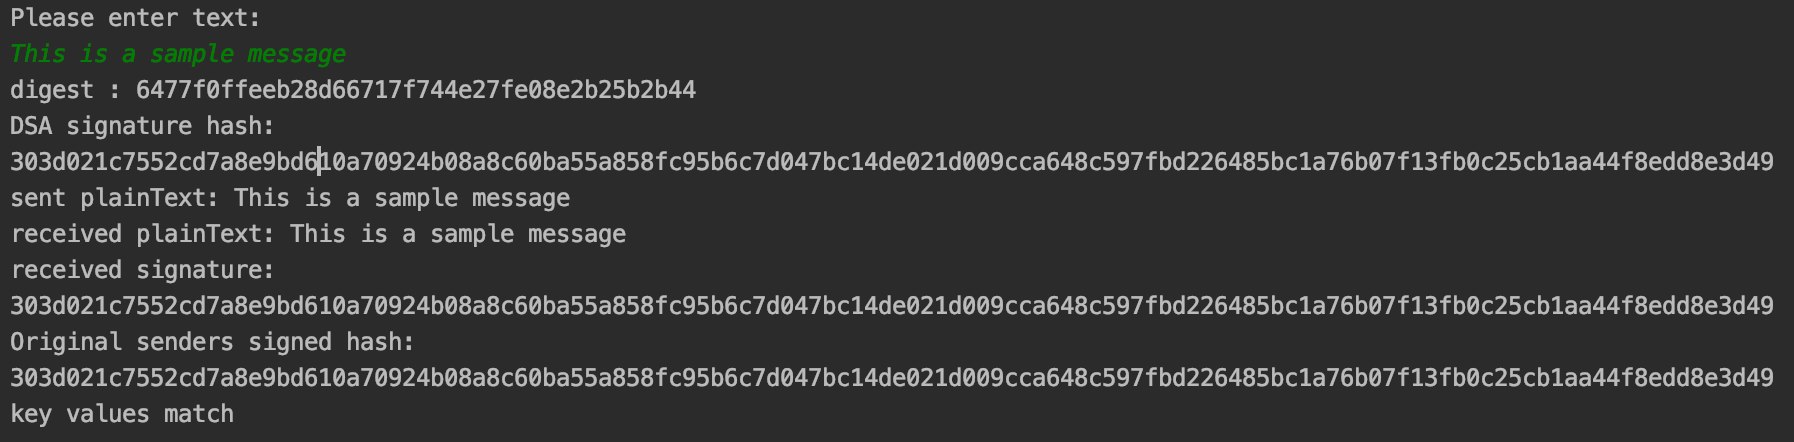
\includegraphics[scale=0.5]{Images/successDSAMessage.png}
  \caption{Output of non intercepted message}
\end{figure}

\textit{Figure 5.} Shows that when the message has been manipulated then the hash that is produced is different and the comparison of keys at the verify function is incompatible and the message cannot be trusted. \\

\begin{figure}[H]
	\centering
	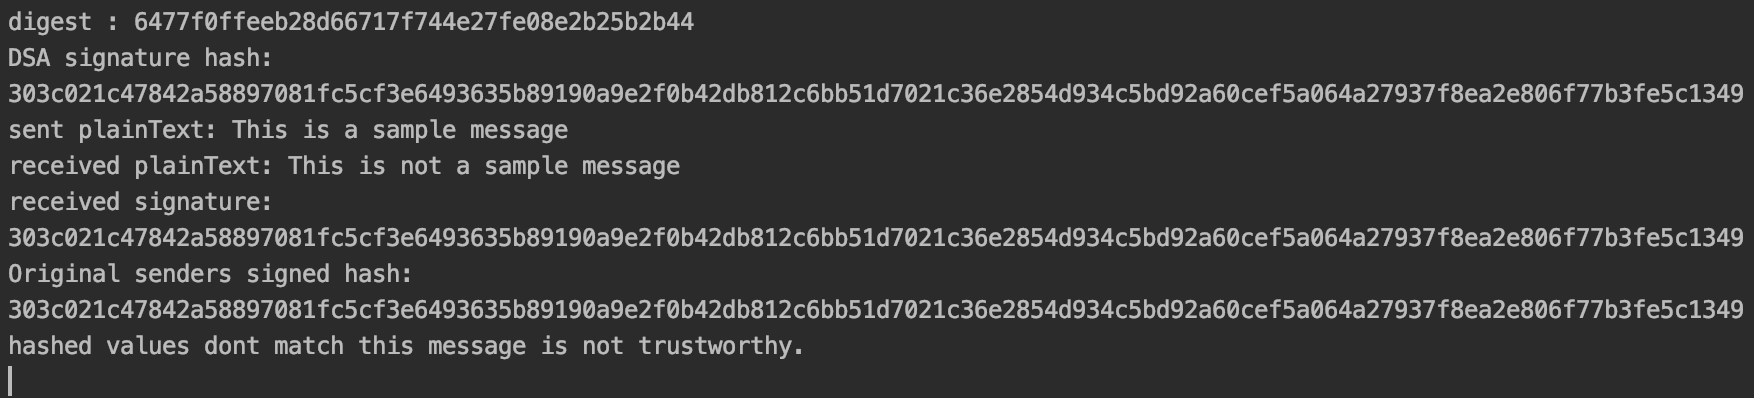
\includegraphics[scale=0.5]{Images/interceptedDSAMessage.png}
  \caption{Output of intercepted message detection}
\end{figure}

\textit{Figure 6.} Shows that even if the original message is the same but the signed hash has been manipulated then the DSA algorithm throws and exception because of the incompatible signature and some form of manipulation has taken place therefore the message is untrustworthy. \\

\begin{figure}[H]
	\centering
	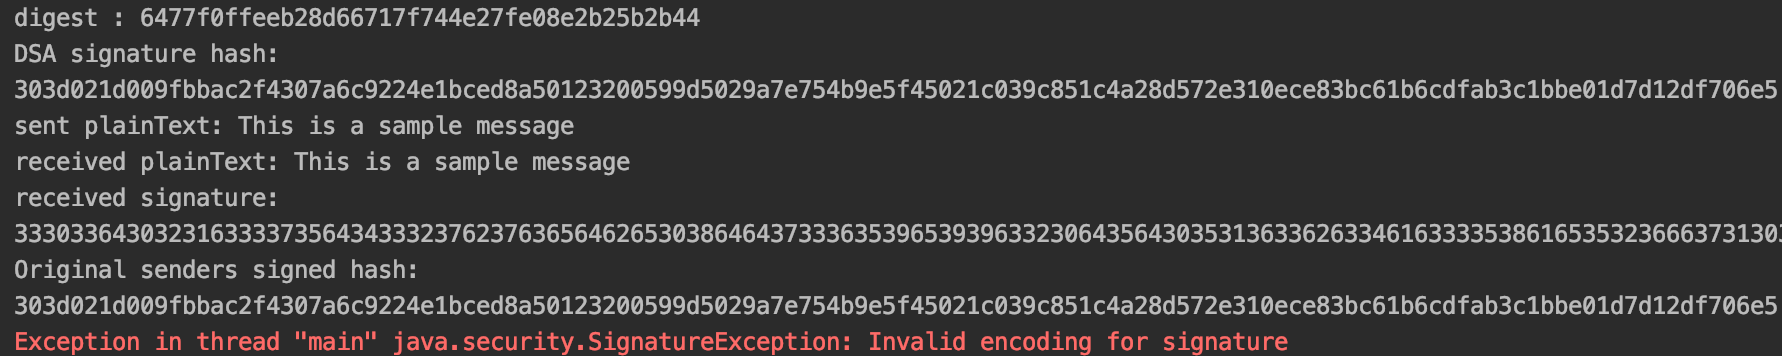
\includegraphics[scale=0.5]{Images/interceptedKeyMessage.png}
  \caption{Output of intercepted message with bad signature detection}
\end{figure}

The advantages of the DSA algorithm are that all keys are generated locally at each sender which means the keys can easily be changed if a key is believed to have been compromised which enhances the security of communications. Another advantage of the DSA algorithm is that it is relatively easy to implement especially if using the JPA toolset.

A disadvantage of the algorithm is that it can be computationally expensive especially if generating new keys for every message sent.


\subsection{HMAC-SHA256 method}
MAC(Message Authentication Code) is another method of message authentication, the HMAC-SHA256 method is very similar to the Hash Functions that are discussed above in \textit{Section 1.1}. The purpose of a MAC like all method authentication methods is to ensure that when messages are passed between 2 parties they are passed without interference or manipulation. If a message has been interfered with or manipulated then the receiver should be able to identify this and can subsequently not trust the message they have received.\\
\\
 - MAC functions assume that a shared key has already been generated and shared between sender and receiver. \\
\\
 - The sender then takes their plain text message and generates a MAC  using the shared private key. This MAC is then used as a tag like in the hashing functions already discussed. The sender then sends the MAC and the original message to the receiver.\\
\\
 - Once the receiver receives the message they take the plain text that has been received and the  the private key which was already shared and generate a MAC themselves.\\
\\
 - The receiver then compares the received MAC and the one they generated to see if the message has been interfered with. If the MAC has been manipulated then the MACs wont match and the message is untrustworthy. Likewise if the message has been changed then the hash generated by the receiver wont match the hash from the sender and the message is untrustworthy. As has previously been discussed in the previous sections the only way for the messages to be considered trustworthy is if the MACs generated by both sender and receiver match. \\

An advantage of MAC is that like hash functions the MAC is considered to be a one way hash function because MAC functions are not reversible. However a disadvantage is that the MAC algorithm requires that the sender and receiver share a secret key. If the secret key becomes compromised then they will both need to share a new secret together which can introduce an overhead. 

\section{Diffie-Hellman with 4 parties}
\subsection{Design for the Diffie-Hellman Protocol}
Following the principles of the Diffie Hellman Protocol means that in order
to read the messages that are being transmitted every party needs to know the
public key of all of the other members in the network in order to generate a shared secret key.

The process is largely the same when more parties are added however because more parties have been added it means that more keys need to be generated and shared. Each party starts the process by using the shared prime number ($q$) and the shared primitive root ($\alpha$ of $q$).

Each key then generates their public keys using an random integer that they have generated. \\
\\
$Y_A = \alpha^{X_A}$ mod q \\
$Y_B = \alpha^{X_B}$ mod q \\
$Y_C = \alpha^{X_C}$ mod q \\
$Y_D = \alpha^{X_D}$ mod q \\

The above keys are then shared among all members of the network and then
then the following calculations are performed in order to calculate the shared secret keys which enables secure communication between all parties in the network\\
\\
A calculates K = $(Y_{BCD})^{X_A}$ mod q \\
B calculates K = $(Y_{ACD})^{X_B}$ mod q \\
C calculates K = $(Y_{ABD})^{X_C}$ mod q \\
D calculates K = $(Y_{ABC})^{X_D}$ mod q \\


\textit{Figure 6.} is an example of the stages that each member of the network goes through in order to finally reach a shared secret key. 

\begin{figure}[H]
	\centering
	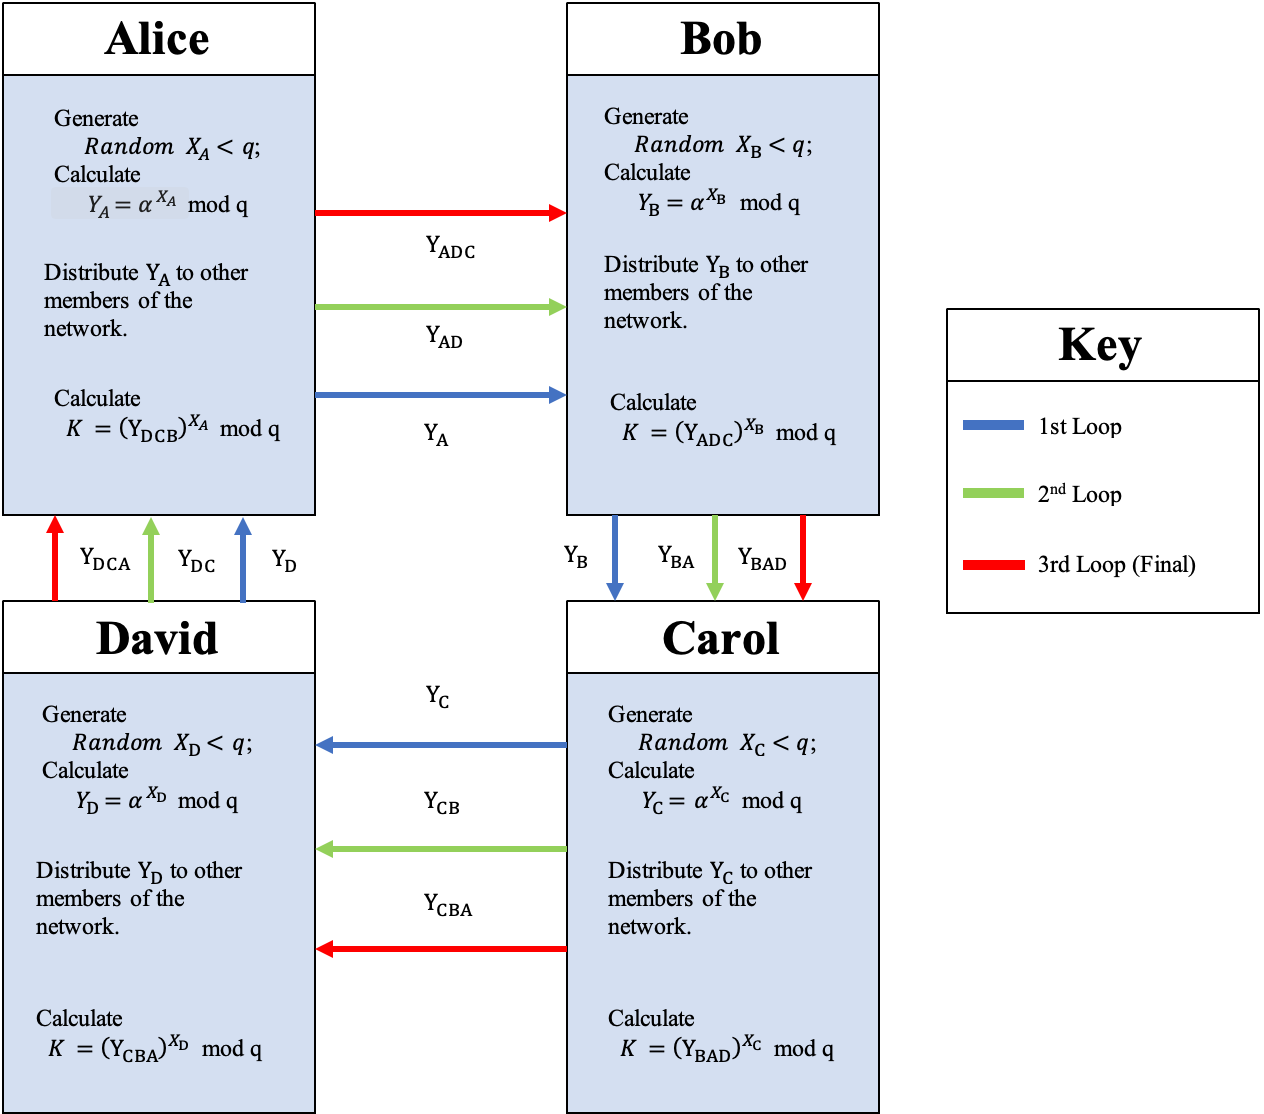
\includegraphics[scale=0.6]{Images/keyExchange.png}
  \caption{Diagram of how keys are passed between members of network.}
\end{figure}


\subsection{Implementation of the Protocol with 4 Parties}
As discussed above in section 2.1 and can be seen from the code in \textit{Appendix F. } I have had to exchange all of the keys amongst each of the members in the network. I have done this through multiple iterations (phases) of the network in order
for everyone within the network to have all of the keys needed to successfully generate a shared secret key for decoding messages that are sent. 
\textit{Figure 7.} shows the iteration cycle of how keys are exchanged over multiple iterations.
\begin{center}
  \captionof{table}{Table outlining the order in which the keys are gathered in the Diffie-Hellman exchange.}
	\begin{tabular}{ |c|l|l|l|l| } 
	 \hline
	 \multicolumn{1}{|c|}{}& \multicolumn {4}{|c|}{Public Keys held by network members} \\
	 \hline
   N & Alice & Bob & Carol & David \\
   \hline
   0 & A & B & C & D \\
   1 & AD & BA & CB & DC \\
   2 & ADC & BAD & CBA & DCB \\
   3 & ADCB & BADC & CBAD & DCBA \\
	 \hline
  \end{tabular}
\end{center}
\pagebreak

\textit{Table 1.} above details how the keys are gathered within the program. In iteration 0 the only keys that each members have are their own however as we iterate around the network the keys are gathered until every member has every other members public keys. Once every member has all of the other members public keys they are able to calculate the shared secret for the decoding of all messages. This is displayed in the code output(\textit{Appendix G}) via printing the secrets generated by each individual member and then comparing the keys. If the keys do not match then the program with throw an error however if all keys match the output should be the same as \textit{Appendix G} which shows that all parties within the program share the same secret key and can therefore communicate amongst each other. 

\newpage
\section*{Appendices}
\appendix
\section{SHA1 Message Digestor}
\textbf{Note:} This small digestor is used within the example for RSA Encryption with SHA-1 Hashing (\textit{Appendix B} \& \textit{Appendix C}).
\lstinputlisting{../RSAEncryptionSHA1/src/MessageDigestor.java}
\newpage
\section{RSA Encryption + SHA1 Hash Sender Program}
\textbf{Note:} This program is the code for the sender section of the RSA + SHA1 method. This method calls its counterpart verifier program \textit{Appendix C} passing in the message sent to the verifier.
\lstinputlisting{../RSAEncryptionSHA1/src/Sender.java}
\newpage
\section{RSA Encryption + SHA1 Hash Verifier Program}
\lstinputlisting{../RSAEncryptionSHA1/src/Verifier.java}
\newpage
\section{DSA Sender Program}
\lstinputlisting{../DSA/src/Sender.java}
\newpage
\section{DSA Verifier Program}
\lstinputlisting{../DSA/src/Verifier.java}
\newpage
\section{Diffie Hellman 4 Party Key Exchange}
\lstinputlisting{../Diffie_Hellman/src/DHKeyAgreement4.java}
\newpage
\section{Diffie Hellman 4 Party Output}
\textbf{Note:} If you would like to print the keys out in order to visually compare them yourself you can change this with the boolean flag in the code base. Change the variable \textit{showKeys} to false and then compile and run the program again. \\
\\
These Instructions assume you are compiling from the directory that the code file is in.\\
\textbf{Compile:}javac ./DHKeyAgreement4.java \\
\textbf{Run:}java DHKeyAgreement4
\\
\\
\textbf{Output:}
\lstinputlisting{./Files/DHKeyAgreement4_output.txt}

\end{document}